\section{Vergleich der Wirkunsgrade}
Bei der Aachen-Turbine ergaben sich je nach Berechnungsart folgende Werte für den Wirkungsgrad:
\begin{table}[H]
	\centering
	\caption{Wirkungsgrad bei der Aachen-Turbine}
	\begin{tabular}{ c| c | c}
Berechnungsformel	&	$\eta_{strukturiert}$	&	$\eta_{unstrukturiert}$	\\
\hline
1 Stufe	&		&		\\
\hline
$\eta_{CFX}$	&	$92,33\%$	&	$92,23\%$	\\
$\eta_{c_p, T_t}$	&	$92,44\%$	&	$92,23\%$	\\
$\eta_{torque}$	&	$92,87\%$	&	$90,58\%$	\\
\hline
1,5 Stufen 	&		&		\\
\hline
$\eta_{CFX}$	&	$86,42\%$	&	$87,05\%$	\\
$\eta_{c_p, T_t}$	&	$86,48\%$	&	$87\%$	\\
$\eta_{torque}$	&	$87.05\%$	&	$85,58\%$	\\

	\end{tabular}
	\label{tab:wgaachen}
\end{table}
In Tabelle \ref{tab:wgaachen} werden die Wirkungsgrade des strukturierten und des unstrukturierten Gitters dargestellt. Diese weichen höchstens um $1,7\%$ voneinander ab. Es ist zu erkennen, dass die Wirkungsgrade im strukturierten Fall bei einer Stufe bis zu zwei Prozentpunkten größer sind. Bei der Betrachtung von 1,5 Stufen ist dagegen zu erkennen, dass die Wirkungsgrade im strukturierten Fall um $0,6$ Prozentpunkte kleiner sind.\\
Dies kann an dem Übergang vom Rotor in den zweiten Stator liegen. Dort findet ein Wechsel des Gitters von unstrukturiert nach strukturiert statt.\\
Allerdings ist die durchgeführte Gitterstudie im unstrukturierten Fall nicht zufriedenstellend durchgeführt, was in den Abbildungen \ref{fig:gitterunstrukturiert1stufe} und \ref{fig:gitterunstrukturiert15stufen} zu erkennen ist. Daher fällt ein Vergleich der beiden Gittertypen schwer und ist nicht aussagekräftig. \\ 

Aus den physikalischen Grundlagen zur Berechnung des Wirkungsgrades ist nach dem Satz der Massenerhaltung der Massenstrom über die gesamte Turbine konstant.
Aufgrund numerischer Faktoren, sowie konstruktionsbedingt kann es jedoch zu Veränderungen im Massenstrom kommen. 
Insbesondere kommt es an den Verbindungsstellen der einzelnen Domänen zu Abweichungen. Hierzu wird in Kapitel \ref{cha:kanal} näher eingegangen.
Auffällig ist jedoch, dass es hierbei gravierende Unterschiede im Hinblick auf die Gitterstrukturierung gibt. In Abbildung \ref{fig:massFlowUnstrukt} ist der Verlauf des Massenstroms durch die Turbine dargestellt. Die Position in der Turbine ist auf der Abszisse dargestellt, die Interfaces befinden sich bei 1 und 2. Auf der Ordinate ist der jeweilige Massenstrom aufgetragen. Für die unstrukturierte Vernetzung treten Massenstromunterschiede von $0,1664 \frac{kg}{s}$ auf. Im Vergleich dazu liegt die Massenstromabweichung für das strukturierte Gitter, siehe Abbildung \ref{fig:massFlowStrukt}, lediglich bei $0.00028\frac{kg}{s}$.

 \begin{figure}[htbp]
	\centering
	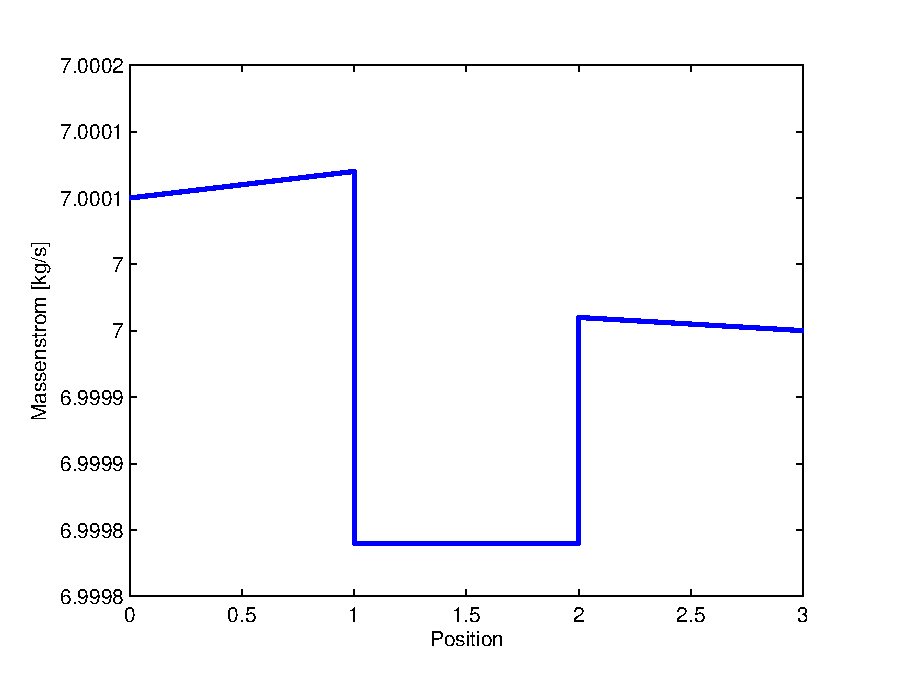
\includegraphics[width=0.8\textwidth]{massFlow_strukt.eps}
	\caption{Massenstrom über in der Turbine, strukturiertes Gitter} \label{fig:massFlowStrukt}
\end{figure} 
 \begin{figure}[htbp]
	\centering
	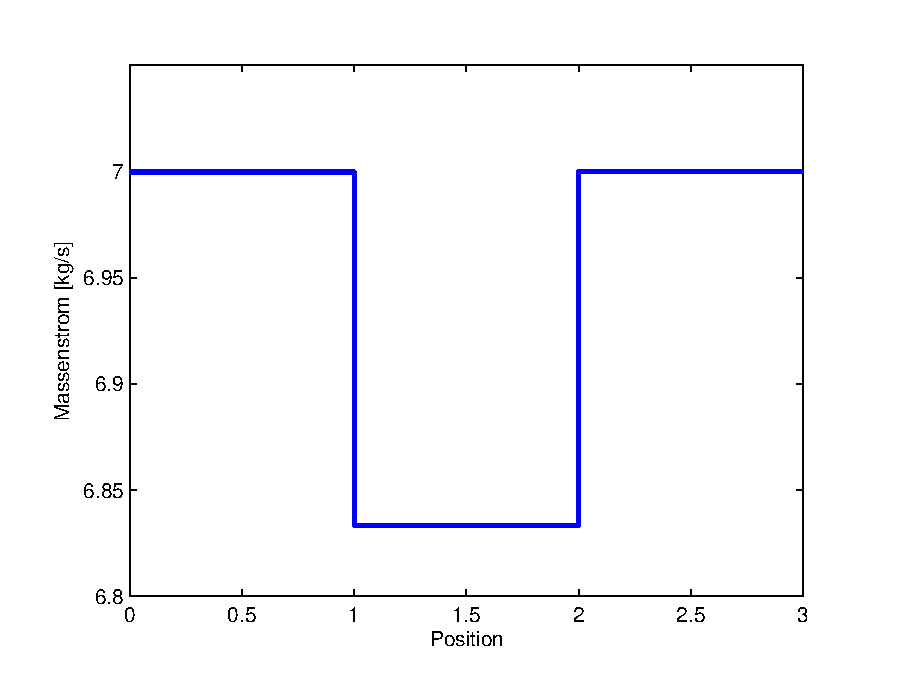
\includegraphics[width=0.8\textwidth]{massFlow_unstrukt.eps}
	\caption{Massenstrom über in der Turbine, unstrukturiertes Gitter} \label{fig:massFlowUnstrukt}
\end{figure} 
\subsubsection{Wirkungsgrade mit temperaturabhängigem $c_p$}
\begin{table}[H]
	\centering
	\caption{Vergleich der Wirkungsgraddefinitionen auf einem strukturierten Gitter mit $c_p = f(T)$}
	\begin{tabular}{ l| c | c c c c}
		&	$c_p = const.$	&	$c_p(T)$	&		&		&		\\
		\hline
		&		&	CpIs	&	Ave CpIS	&	Ave	&	mycp	\\
		\hline
		$\eta_{CFX}$	&	81,24 \%	&	53,89\%	&	79,19 \%	&	79,19 \%	&	60,25\%	\\
		$\eta_{c_p, T_t}$	&	81,25\%	&	74,6 \%	&	78,3 \%	&	78,07\%	&	83,41 \%	\\
	$\eta_{torque}$	&	82,52\%	&	54,35 \%	&	80,11 \%	&	79,87 \%	&	60,77\%	\\
		
	\end{tabular}
	\label{tab:strukturiertmycp}
\end{table}

\begin{table}[H]
	\centering
	\caption{Vergleich der Wirkungsgraddefinitionen auf einem unstrukturierten Gitter mit $c_p = f(T)$}
	\begin{tabular}{ l| c | c c c c}
		&	$c_p = const.$	&	$c_p(T)$	&		&		&		\\
		\hline
		&		&	CpIs	&	Ave CpIS	&	Ave	&	mycp	\\
		\hline
		$\eta_{CFX}$	&	80,21 \%	&	71,93 \%	&	77,96 \%	&	78,34 \%	&	60,01 \%	\\
		$\eta_{c_p, T_t}$	&	80,1 \%	&	\textcolor{red}{100,36} \%	&	78,23 \%	&	78,61\%	&	83,72 \%	\\
		$\eta_{torque}$	&	79,5 \%	&	70,23 \%	&	77,1 \%	&	77,48 \%	&	59,36 \%	\\
		
	\end{tabular}
	\label{tab:unstrukturiertmycp}
\end{table}